\providecommand{\main}{..}
\documentclass[\main/main.tex]{subfiles}
\begin{document}

\chapter{Probabilità}
\section{Disuguaglianza di Chernoff}
\begin{figure}
  \[
    \prob{\abs{X_{n,p} - np} \geq n\epsilon} < 2e^{-2\epsilon^2 n}
  \]
  \caption{Disuguaglianza di Chernoff per le binomiali}
\end{figure}
La \textbf{disuguaglianza di Chernoff} è utilizzata quando è necessario calcolare la probabilità di una \textbf{funzione} \(f\) che:
\begin{enumerate}
  \item Non è semplice da calcolare, oppure,
  \item Non è nota.
\end{enumerate}

\subsection{Caratteristiche}

Possiede 3 distinte caratteristiche:

\subsubsection{Variabili di indipendenti}
Essa richiede che le \textbf{variabili siano indipendenti}, \textit{condizione che la disuguaglianza di Markov non richiede} e nel caso delle disuguaglianza di Chebyshev è necessaria solo l'indipendenza da coppie di variabili casuali.

\subsubsection{Non è una disuguaglianza “vera“}
La disuguaglianza di Chernoff \textbf{non è una disuguaglianza vera}, ma piuttosto va vista come una tecnica per ottenere limiti esponenziali decrescenti sulle probabilità di coda.

\subsubsection{Il valore di \(n\) è arbitrario}
La disuguaglianza di Chernoff non fornisce un preciso valore di \(n\) oltre il quale siamo sicuri che la probabilità della coda sia minore di una \(\delta \) fissata.

\subsection{Applicazioni alle binomiali}
Nell'analisi degli algoritmi probabilistici occorre spesso valutare la coda di una binomiale, ovvero la probabilità che questa variabili aleatoria disti dalla media per una quantità fissata.

Partendo dalla \textbf{disuguaglianza di Chebyshev} per una variabile \(X\) con \(\Var{X}\) finita:

\begin{figure}
  \[
    \prob{\abs{X-\mean{X}} \geq a} \leq \frac{\Var{X}}{a^2} \quad \forall a > 0
  \]
  \caption{Disuguaglianza di Chebyshev}
\end{figure}

\begin{figure}
  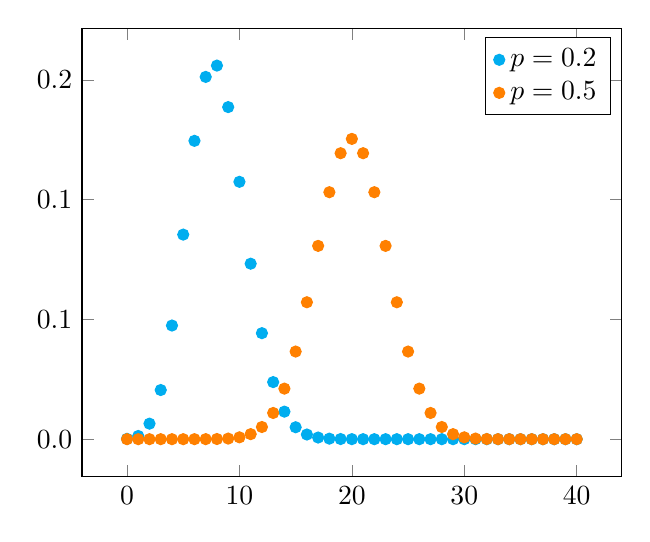
\begin{tikzpicture}[
      declare function={binom(\k,\n,\p)=\n!/(\k!*(\n-\k)!)*\p^\k*(1-\p)^(\n-\k);}
    ]
    \begin{axis}[
        samples at={0,...,40},
        yticklabel style={
            /pgf/number format/fixed,
            /pgf/number format/fixed zerofill,
            /pgf/number format/precision=1
          }
      ]
      \addplot [only marks, cyan] {binom(x,40,0.2)}; \addlegendentry{$p=0.2$}
      \addplot [only marks, orange] {binom(x,40,0.5)}; \addlegendentry{$p=0.5$}
    \end{axis}
  \end{tikzpicture}
  \caption{Distribuzioni binomiali al variare del parametro \(p\)}
\end{figure}

Nel caso di \(X_{n,p}\) binomiale, con media \(\mean{X} = np\) e varianza \(\Var{X} = npq\), \(\forall \epsilon > 0\) vale che:

\[
  \prob{\abs{X_{n,p} - np} \geq n\epsilon} \leq \frac{pq}{\epsilon}\cdot \frac{1}{n} = \O{\frac{1}{n}}
\]

Per il \textbf{teorema del limite centrale} vale che:

\[
  \frac{X_{n,p} - np}{\sqrt{npq}} \longrightarrow \normal
\]

Applico il limite ed ottengo:

\[
  \lim_{n\rightarrow+\infty} \prob{\frac{X_{n,p} - np}{\sqrt{npq}}\geq \epsilon} = \frac{2}{\sqrt{2\pi}} \int_{\epsilon}^{+\infty} e^{-\frac{t^2}{2}} dt
\]

Vado ad aggiungere il termine \(\sqrt{\frac{n}{pq}}\) come coefficiente a \(\epsilon \) per consentire l'integrazione:

\[
  \lim_{n\rightarrow+\infty} \prob{\frac{X_{n,p} - np}{\sqrt{npq}}\geq \sqrt{\frac{n}{pq}}\cdot \epsilon} = \frac{2}{\sqrt{2\pi}} \int_{\sqrt{\frac{n}{pq}}\cdot \epsilon}^{+\infty} e^{-\frac{t^2}{2}} dt
\]

Maggioro l'integrale:

\[
  \frac{2}{\sqrt{2\pi}} \int_{\sqrt{\frac{n}{pq}}\cdot \epsilon}^{+\infty} e^{-\frac{t^2}{2}} dt \leq \frac{2}{\sqrt{2\pi}} \int_{\sqrt{\frac{n}{pq}}\cdot \epsilon}^{+\infty} \frac{t}{\sqrt{\frac{n}{pq}}\cdot \epsilon}e^{-\frac{t^2}{2}} dt = \O{\frac{1}{\sqrt{n}} e^{-\frac{\epsilon^2}{2pq}}n}
\]

Il risultato ottenuto, si avvicina allo \(0\) molto più velocemente del valore \(\O{\frac{1}{n}}\) ottenuto precedentemente tramite la disuguaglianza di Chebyshev.

La disuguaglianza di Chebyshev è più generale, di conseguenza è più debole. Per esempio nel caso della distribuzione gaussiana risulta molto debole, per cui se è necessario avere un'accuratezza maggiore conviene assolutamente usare la disuguaglianza di Chernoff.

\subsection{Esempio: Riduzione della probabilità di errore di un algoritmo}
Supponiamo di voler calcolare una funzione \(f_ I \rightarrow O\) difficile da calcolare e di disporre di un algoritmo probabilistico \(\mathcal{A}\) tali che \(\forall x \in I, T_{\mathcal{A}} \leq p\rnd{\abs{x}}\) dove \(p\) è un polinomio di grado \textbf{piccolo} e che \(\prob{A(x) = f(x)} \geq \frac{3}{4}\), col valore di destra maggiore di \(\frac{1}{2}\) e indipendente da \(x\), altrimenti non potrei determinare il risultato corretto la frequenza con cui appare

Dato un intero \(t > 0\), chiamiamo \(\mathcal{A}_t\) l'algoritmo probabilistico che ripete \(\mathcal{A}\) per un numero \(t\) di volte e ne restituisce il valore più frequente, se esso esiste.

L'algoritmo non garantisce che il risultato sia corretto, infatti anche con \(n\) iterazioni rimane possibile che l'algoritmo calcoli con frequenza maggiore la soluzione errata.

\IncMargin{1em}
\begin{algorithm}
  \SetKwInOut{Input}{input}
  \SetKwInOut{Output}{output}
  \Input{\(x \in I\)}
  \Output{Valore più frequente o “non so“}
  \BlankLine
  \Begin{
    \For{\(i \in \sqr{1, \ldots, t}\)}{
      \emph{Esecuzioni indipendenti di \(\mathcal{A}\) su \(x\)}\;
      \(A[i] = \mathcal{A}(x)\)
    }
    \If{\(\exists z \in \rnd{A[1], \ldots, A[t]}: \#\crl{j \in \crl{1, \ldots, t}: z = A[j]} > \frac{t}{2}\)}{
      \Return{z}\;
    }
    \Else{
      \Return{non so rispondere}\;
    }
  }
  \caption{Riduzione della probabilità di errore}\label{algo_disjdecomp}
\end{algorithm}\DecMargin{1em}

\subsubsection{Quante volte devo iterare l'algoritmo per ridurre la probabilità di errore ad un valore \(\delta \)?}
Utilizzando la disuguaglianza di Chernoff per le binomiali ottengo:
\[
  \prob{\mathcal{A}_t \neq f(x)} \leq \prob{X_{t, \frac{3}{4}} \leq \frac{t}{2}} = \prob{X_{t,\frac{3}{4}} - \frac{3}{4}t \leq -\frac{t}{4}} \leq e^{-2\frac{1}{16}t} = e^{-\frac{1}{8}} \leq \delta
\]
Calcolo il logaritmo naturale ed ottengo il valore di \(t\) per \(\delta = 1000^{-1}\).
\[
  t \geq 8\ln{\frac{1}{\delta}} \Rightarrow t \geq 8 \ln{1000} = 24 \ln{10} \approx 56
\]
Se avessimo invece utilizzato la \textbf{disequazione di Chebyshev} avremmo invece ottenuto un risultato molto peggiore:
\[
  \prob{X_{t, \frac{3}{4}} - \frac{3}{4}t \leq -\frac{t}{4}} \leq \prob{\abs{X_{t, \frac{3}{4}} - \frac{3}{4}t} \geq \frac{t}{4}} \leq \frac{3}{t} \Rightarrow t \geq 3000
\]

\subsection{Esempio: Lancio di monete}
Consideriamo il caso di una variabile aleatoria \(X_{n, \frac{1}{2}}\) con media \(\mean{X} = \frac{n}{2}\):
\[
  \prob{\abs{X_{n, \frac{1}{2}} - \frac{n}{2}} \geq \sqrt{n\log{n}}} \leq 2e^{-2\log{n}} = \frac{2}{n^2}
\]
Per esempio, posto \(n=100\) si ottiene:
\[
  \prob{\abs{X_{n, \frac{1}{2}} - 50} \geq 21} \leq \frac{1}{5000}
\]
Rendendo la maggiorazione più aderente, dividendo il termine destro per due, si ottiene:
\[
  \prob{\abs{X_{n, \frac{1}{2}} - \frac{n}{2}} \geq \sqrt{\frac{n\log{n}}{4}}} \leq 2e^{\frac{-2\log{n}}{4}} = \frac{2}{\sqrt{n}}
\]
Nuovamente risolvendo per \(n=100\) si ottiene:
\[
  \prob{\abs{X_{n, \frac{1}{2}} - 50} \geq 10.5} \leq \frac{1}{5} \rightarrow \prob{39 \leq X_{n, \frac{1}{2}} \leq 61} \geq \frac{4}{5}
\]
\subsection{Esempio: Intervalli di confidenza}
Si vuole valutare la probabilità \(p\) di un evento \(A\) disponendo di un test \(f\) sull'evento \(A\) che restituisce un valore:

\[
  f: \begin{cases}
    \text{SI} & \text{con probabilità } p   \\
    \text{NO} & \text{con probabilità } 1-p
  \end{cases}
\]
\(\frac{X_{n,p}}{n} = \bar{p}\) è una variabile aleatoria con media \(\mean{X_{n,p}} = np\).

\[
  \prob{\abs{p-\bar{p}}\geq \delta} = \prob{\abs{np - X_{n,p}}\geq n\delta} \leq 2e^{-2\delta^2 n} \leq t
\]
\[
  -2\delta^2 n \leq \log{\frac{2}{t}} \Rightarrow n \leq \frac{1}{2\delta^2}\log{\frac{2}{t}}
\]
Dove \(t\) rappresenta la probabilità di errore.

Ponendo \(\delta = 0.1\) e \(t = 100^{-1}\) si ottiene:

\[
  n \leq 50\log{200} = 50\rnd{\log{2} + 2\log{10}} \approx 250 \Rightarrow n \geq 250
\]

\end{document}













